\chapter{Delegation}

An important design decision when modeling data is how many Java classes to use to represent an entity. At one extreme, all of the attributes of an entity are represented by a single class, resulting in a coarse-grained design. At the other extreme, a main entity class delegates functionality to other classes, resulting in a fine-grained design.  Delegation is a very popular pattern because of the flexibility it provides. 

Programmers rarely think about memory costs when deciding how to model entities. Yet, the choices made at this design stage impact memory costs significantly. Coarse-grained designs may result in many objects with unused fields. While delegation is sometimes a way to avoid this problem, overly fine-grained data models can result in poor memory health from excessive object header overhead. This chapter explains how to evaluate object granularity design choices from a memory perspective. It begins with the costs of basic objects, and works up to examples from real applications.
  
\section{The Cost of Objects}
\label{sec:CostOfObjects}

There is no Java library method that returns the size of an object. This is by design. Unlike systems languages like C, a Java programmer is not supposed to know either the size of an object or how it is laid out in memory. The JVM, not the programmer, manages storage, and the JVM has freedom to implement its own policy. However, knowing the sizes of objects is necessary for understanding memory requirements and scalability. Fortunately, it is not hard to estimate the size of an object, and a good estimate is usually sufficient for making intelligent choices among design alternatives. You need to know just a few basics, starting with the size of the Java primitive types. These are given in Table~\ref{tab:primitive-sizes}.
\begin{table}
  \centering
 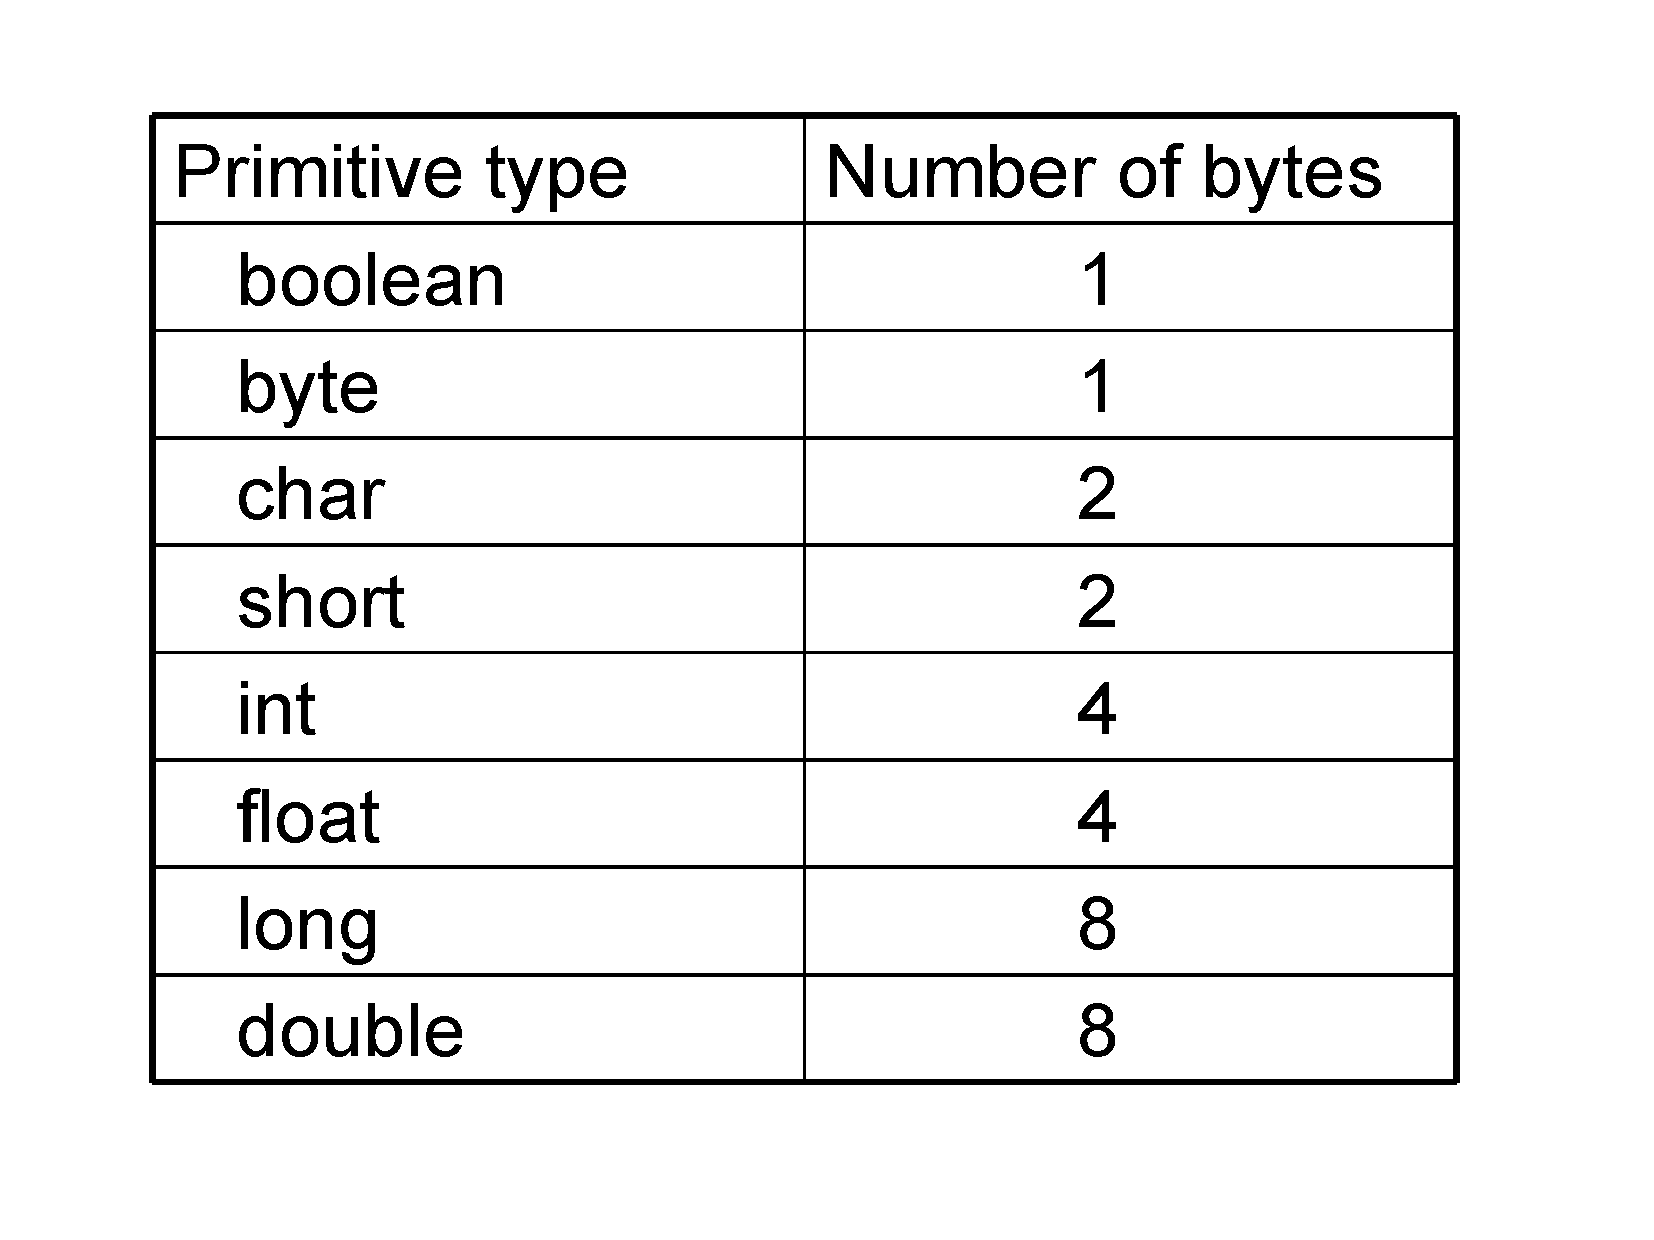
\includegraphics[width=.50\textwidth]{Figures/chapter4/primitive-byte-sizes.pdf}
 % 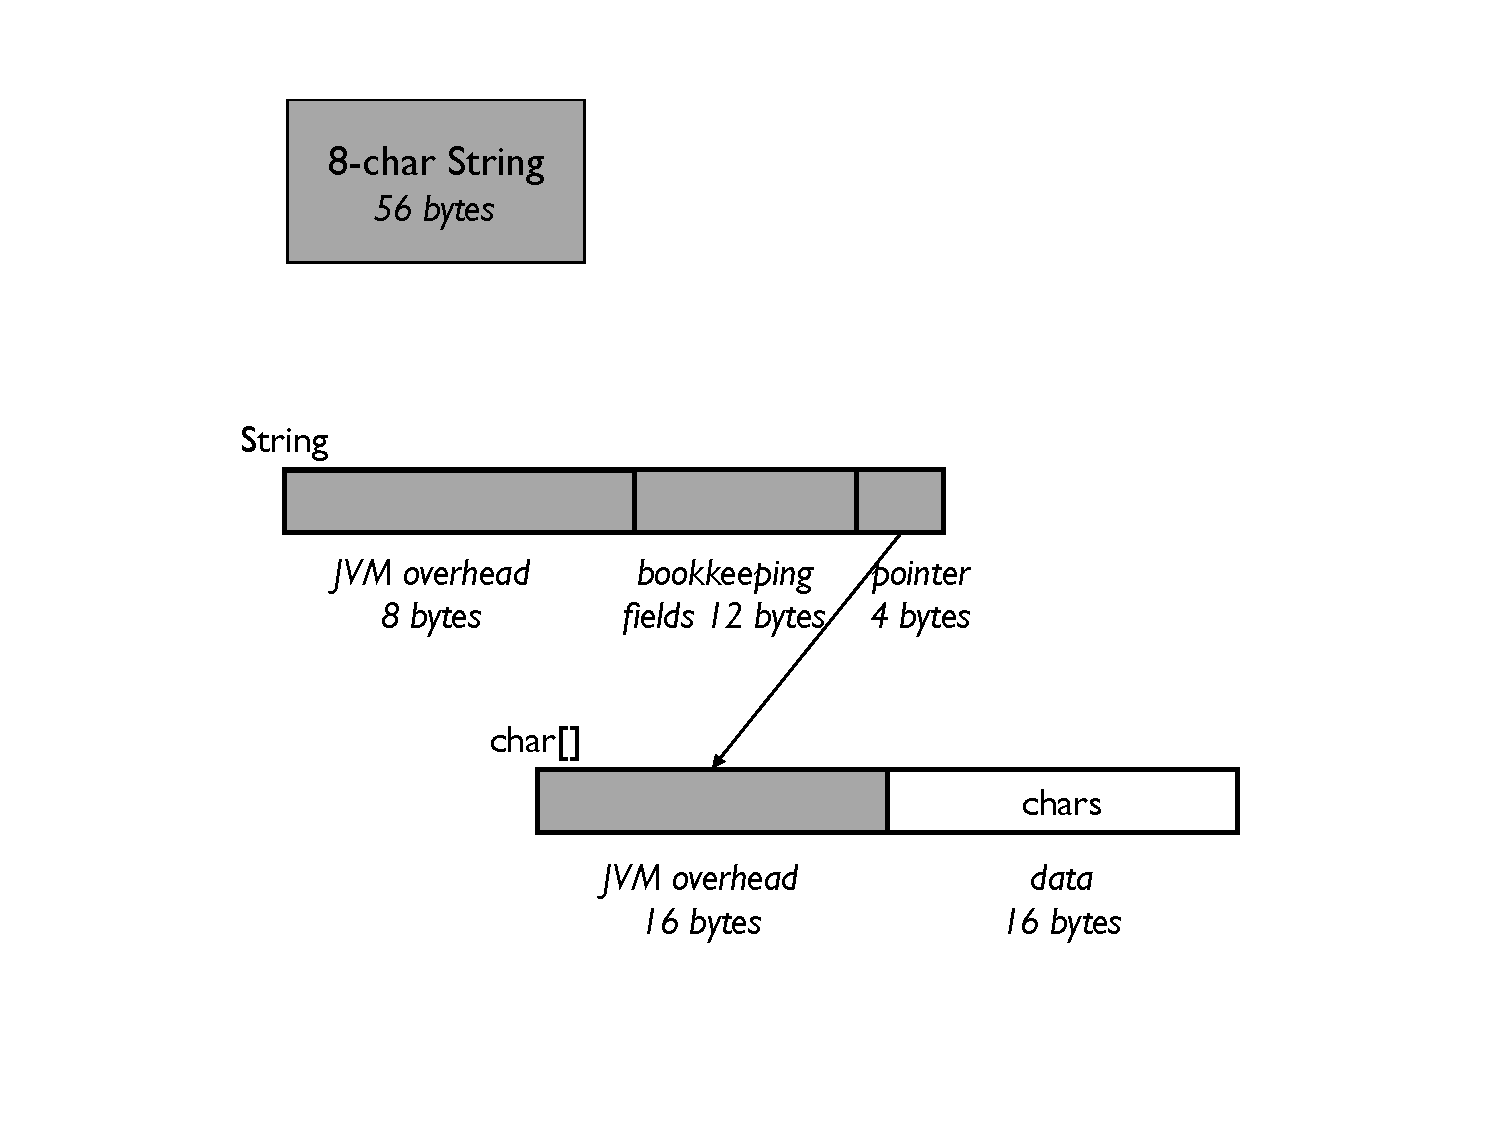
\includegraphics{eight-char-string}
  \caption{The sizes of Java primitive types}
  \label{tab:primitive-sizes}
\end{table}

Objects are much bigger. First, the JVM and the garbage collector require an object header that stores information such as the object's class, a lock, and an identity hashcode. For array objects, the header has an additional integer to store the number of array elements. Secondly, the hardware imposes alignment costs. The hardware may require 2-byte, 4-byte, or 8-byte alignment, depending on the type of the data. For example, integers are usually aligned on a 4-byte boundary, and some hardware might require a double to be aligned on an 8-byte boundary. A JVM may impose additional alignment requirements. This overhead is significant, especially if the object does not have much data in it.

The object header sizes and alignment costs vary depending on the JVM. To illustrate this variability, Table~\ref{tab:object-overhead} gives the costs for both the SUN Java 6 (update 14) JVM and the IBM Java 6 (J9 SR4) JVM. These costs are for 32-bit architectures. It is important to keep in mind that these costs are for specific JVM releases only, and are subject to change in future releases.
\begin{table}
  \centering
 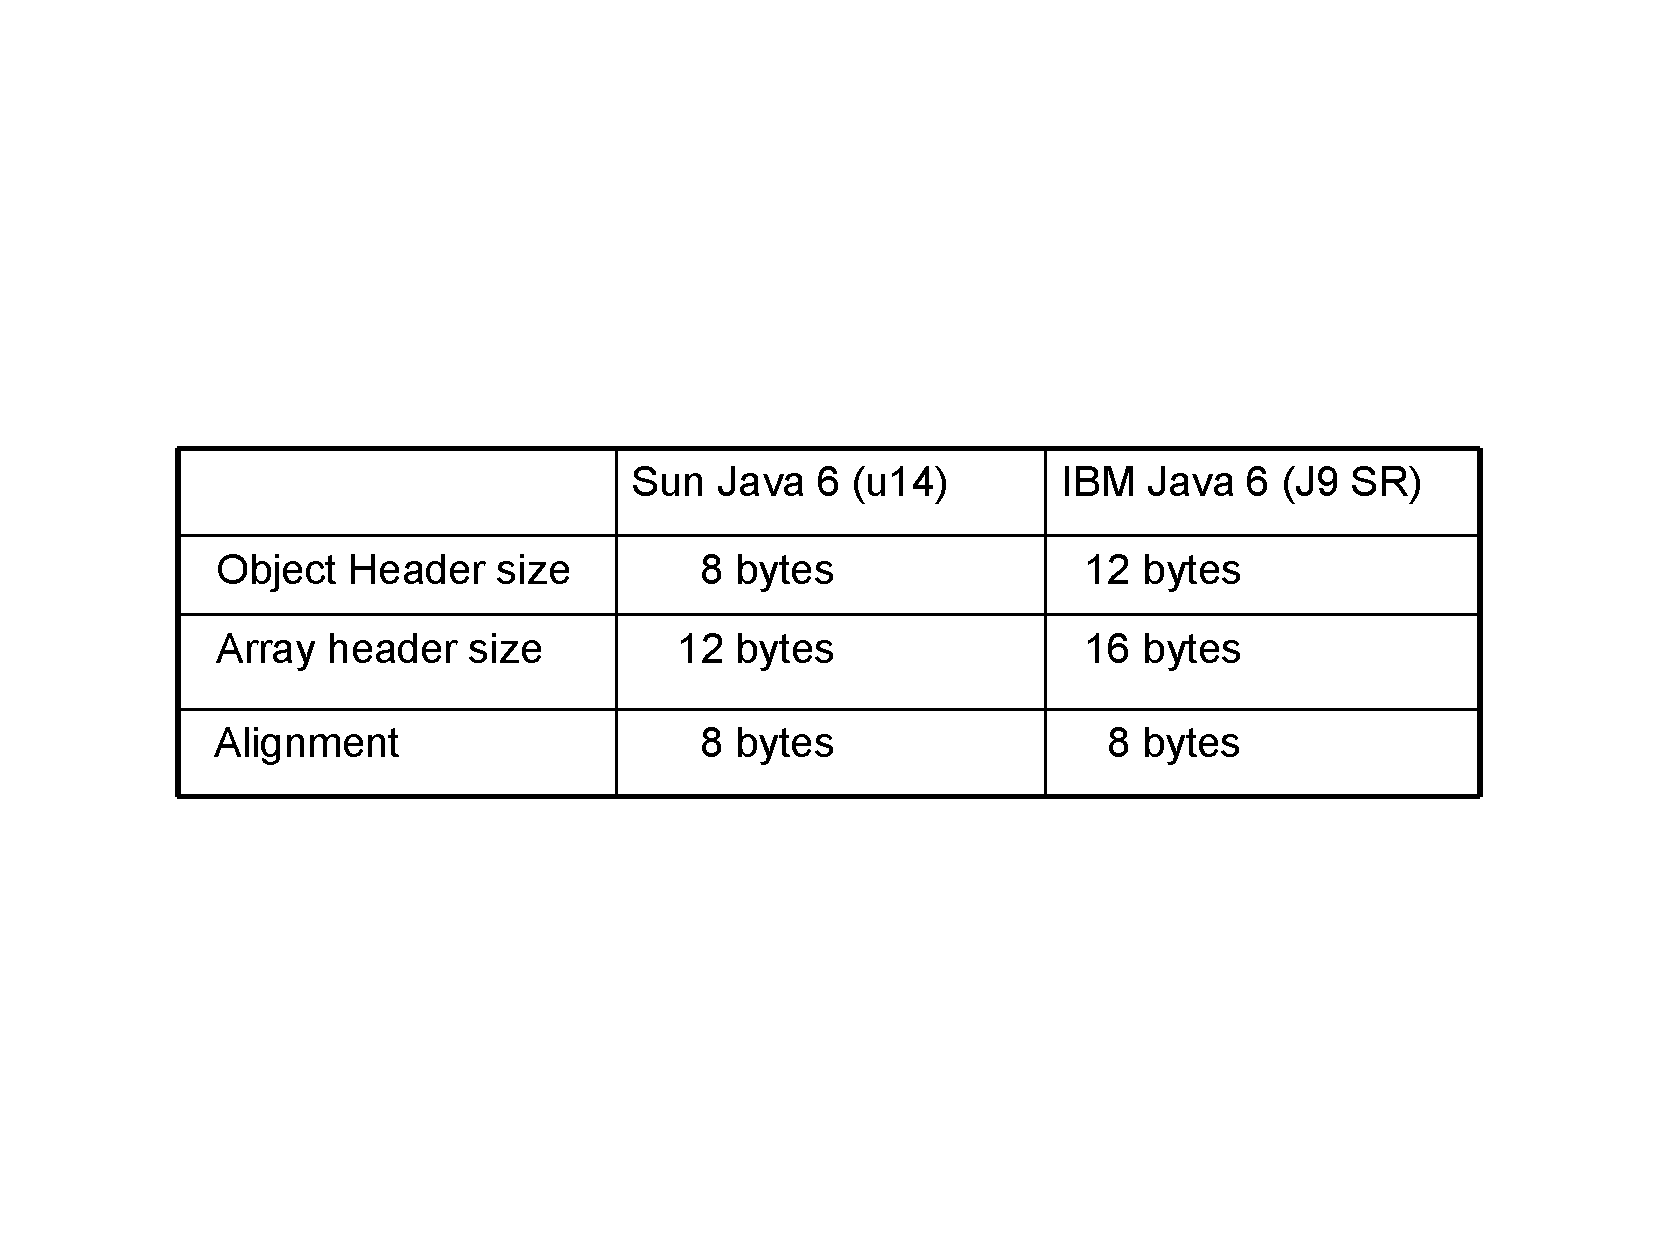
\includegraphics[width=.70\textwidth]{Figures/chapter4/object-overhead.pdf}
 % 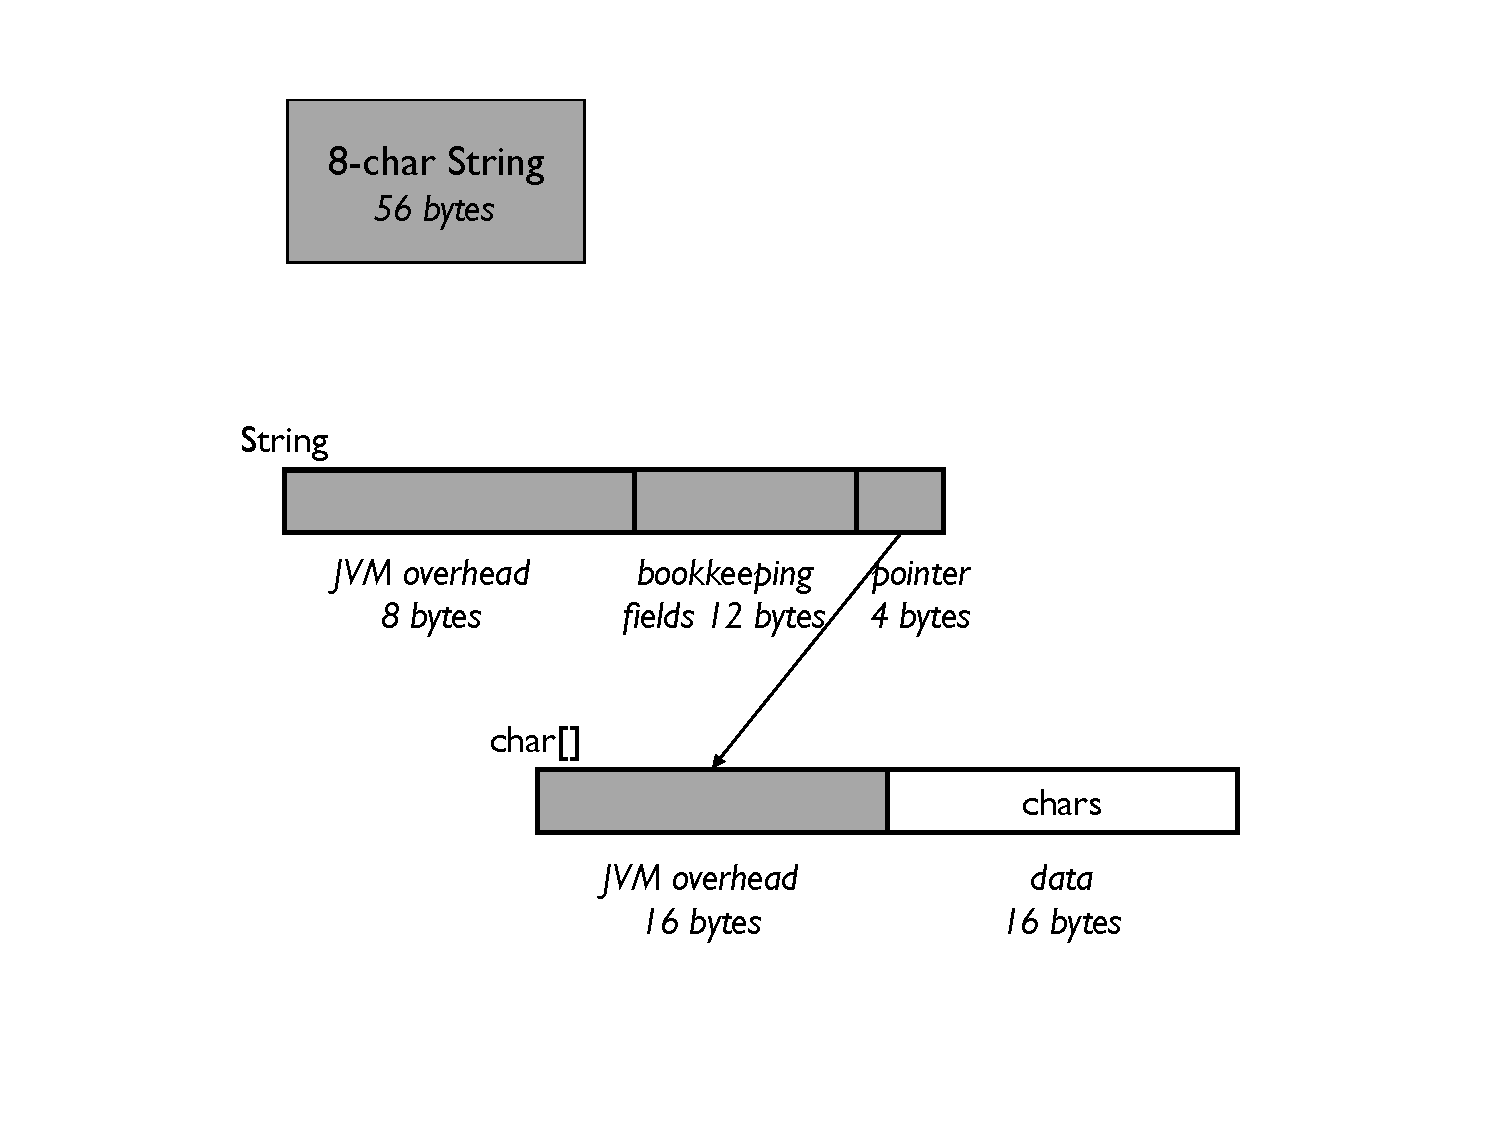
\includegraphics{eight-char-string}
  \caption{The sizes of boxed scalar objects.}
  \label{tab:object-overhead}
\end{table} 
   %The Sun JVM allocates 8 bytes per object header, and the IBM JVM allocates 12 bytes per header. 
 
Boxed scalars, which are objects with a single primitive data type field, are the simplest kind of  object. For both JVMs, a boxed scalar is at least 16 bytes. Since both JVMs allocate objects on 8-byte boundaries, the size of an object must be a multiple of 8. Table~\ref{tab:boxed-scalar-sizes} gives the sizes of boxed scalars.

\begin{table}
  \centering
 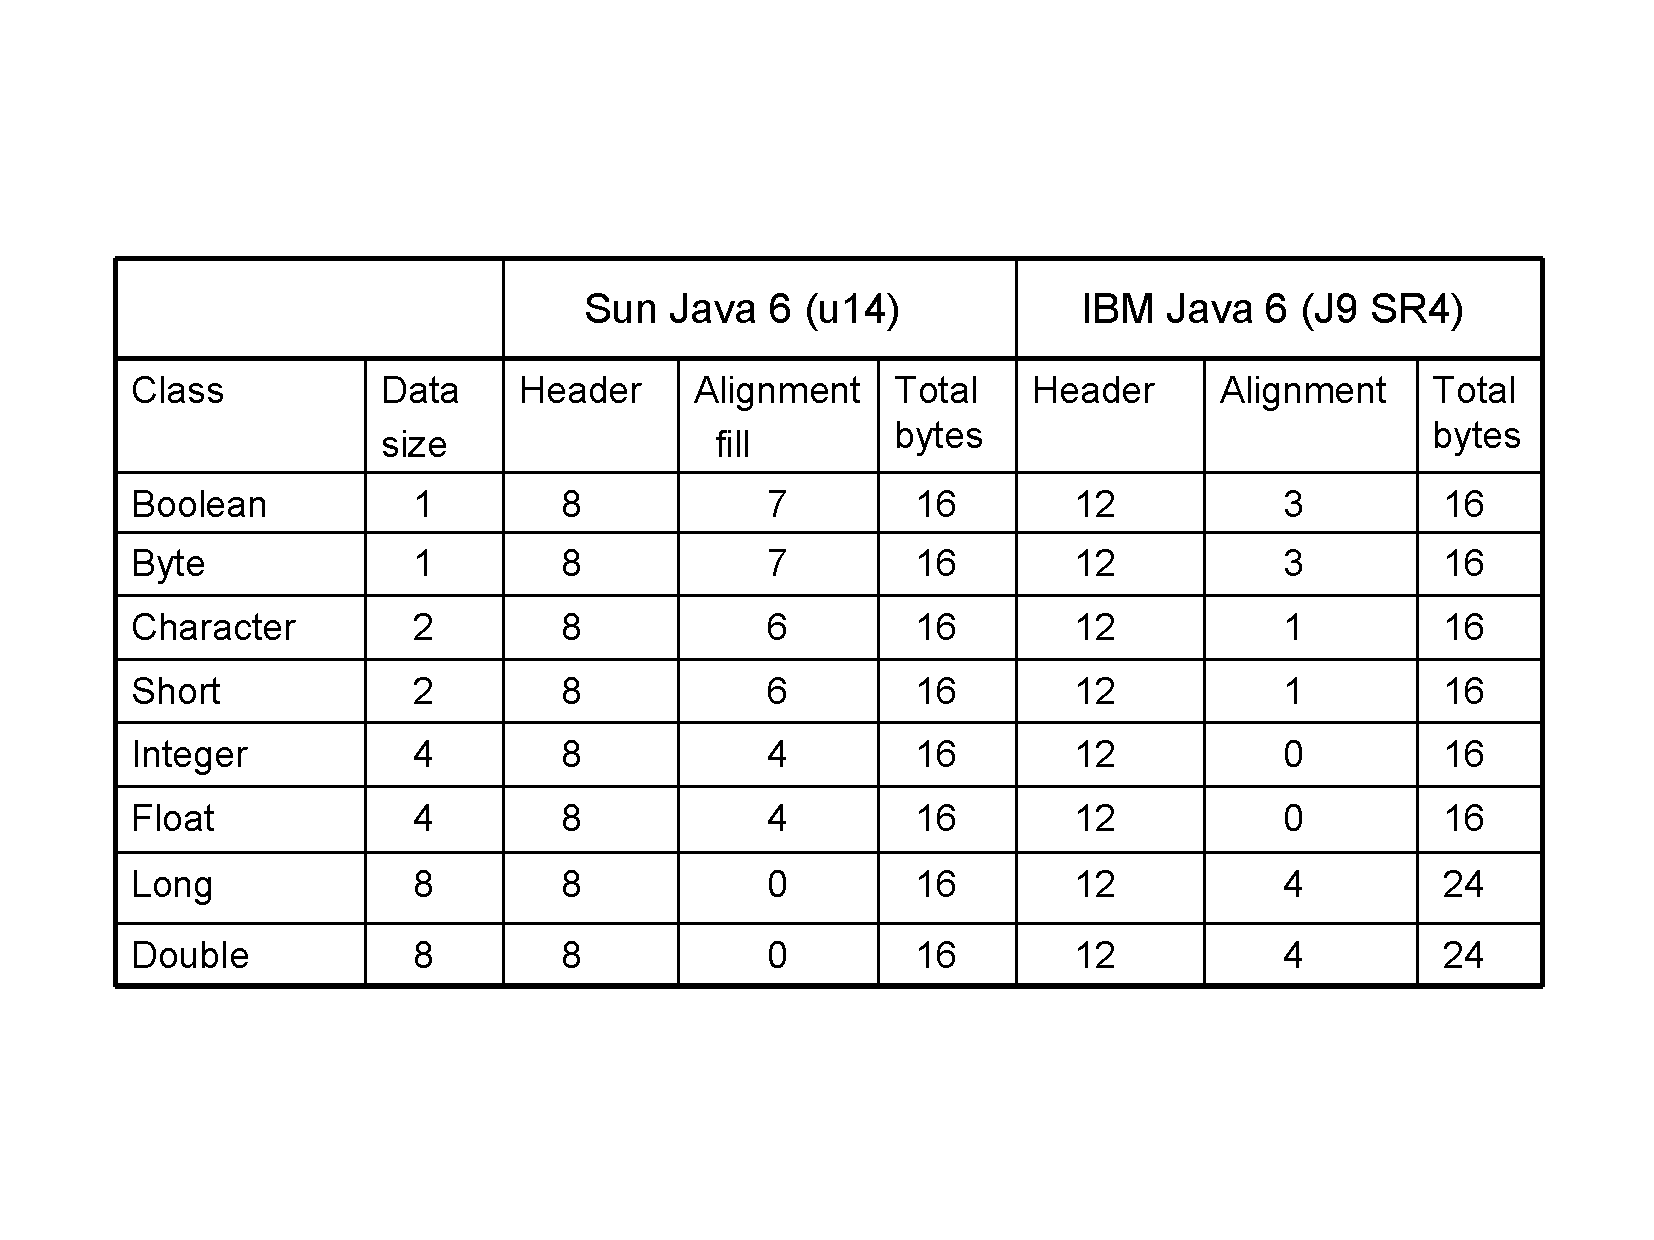
\includegraphics[width=.70\textwidth]{Figures/chapter4/boxed-scalar-sizes.pdf}
 % 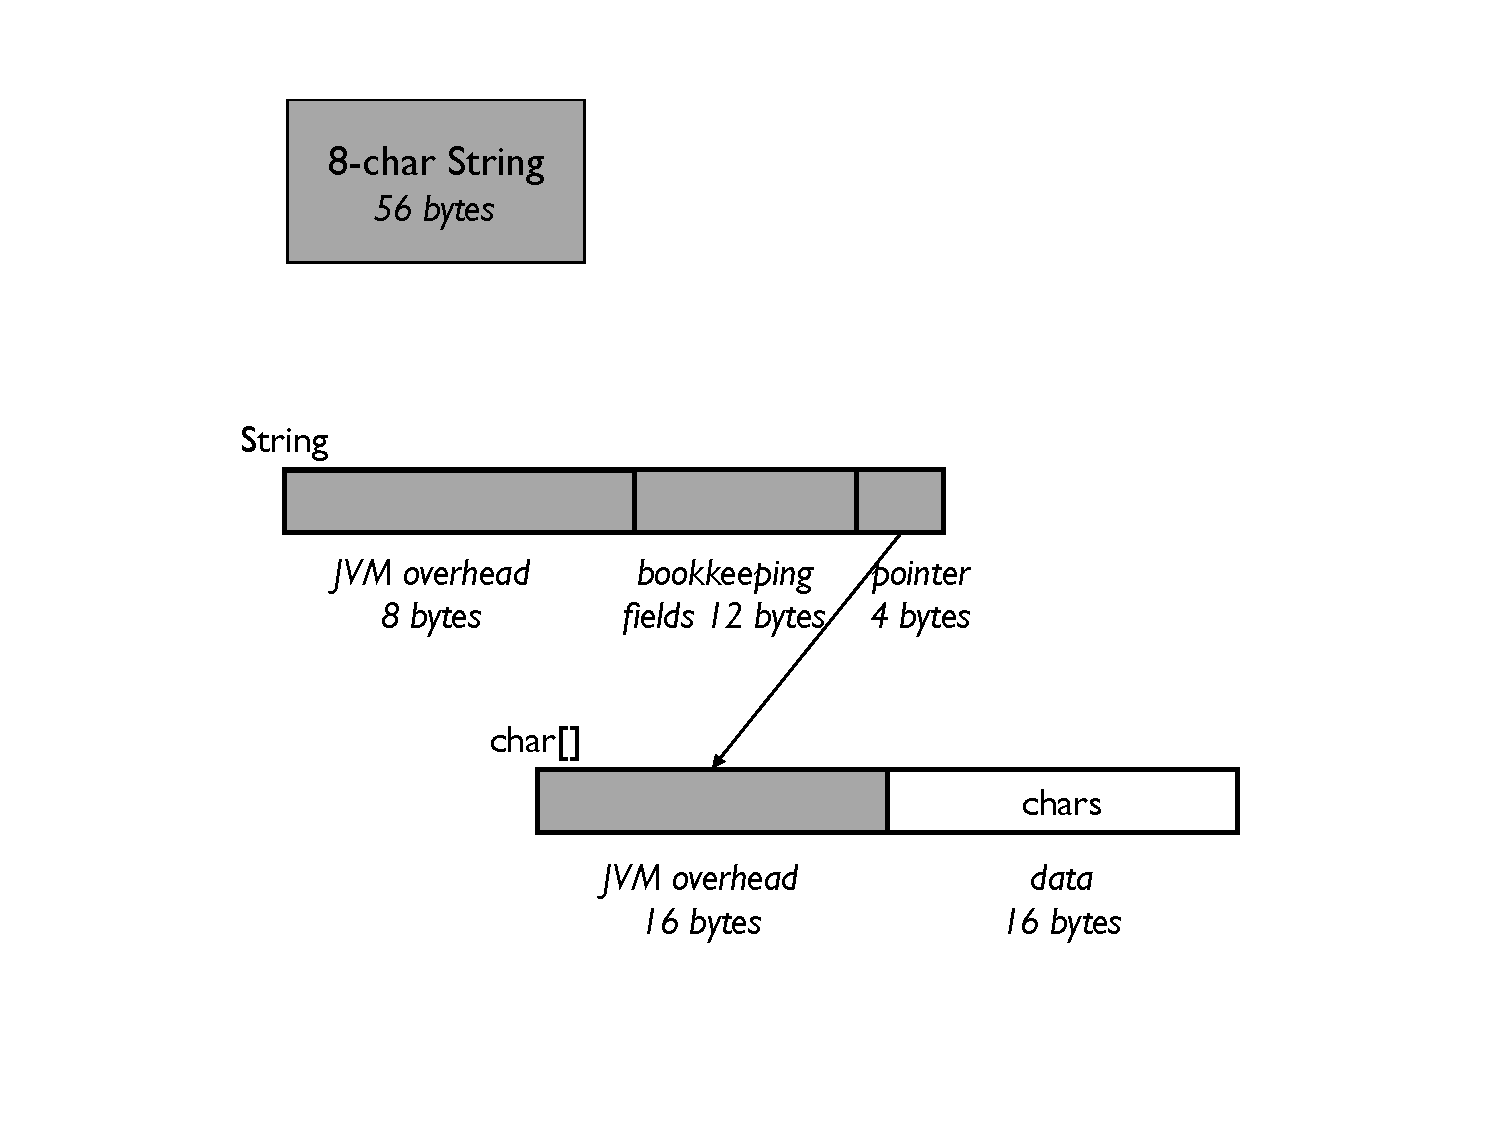
\includegraphics{eight-char-string}
  \caption{The sizes of boxed scalar objects.}
  \label{tab:boxed-scalar-sizes}
\end{table} 

There is a simple rule that holds for boxed scalars. The size of the object is obtained by summing the size of the header and the data, and then rounding it up to the nearest multiple of 8. The generalization of this rule gives you a good way to estimate the size of any object. Often, this estimate turns out to be the real object size, but not always.
 
\callout{callout:minimum-size-estimation-rule}{Minimum-Size Estimate Rule}{
    Let $Header: /gsa/yktgsa/projects/n/nickm-cvs/cvs_repos/papers/bloatbook/Attic/chapter4.tex,v 1.1 2009/08/10 19:06:24 nickm Exp $ be the size of an object header required by the JVM, and $Alignment$ be the object alignment. That is, every object must be allocated at an address which is a multiple of $Alignment$. To estimate the minimum size of an object 1) sum up the sizes of all of its fields, including fields from superclasses, 2) add $Header: /gsa/yktgsa/projects/n/nickm-cvs/cvs_repos/papers/bloatbook/Attic/chapter4.tex,v 1.1 2009/08/10 19:06:24 nickm Exp $ to this sum, and 3) round the result up to the next multiple of $Alignment$. The estimate is exact if the JVM packs and rearranges fields to fit into the smallest space. Otherwise, the actual size can be bigger than the estimated size.
}

\begin{example}[Simple employee class.]
Consider an \texttt{Employee} class with all primitive fields:

\ttfamily
\begin{verbatim} 

			class Employee {
        int hoursPerWeek;
        boolean exempt;
        double salary;
        char jobCode;
        int yearsOfService;
			}
\end{verbatim}
\normalfont
Assume both $Header: /gsa/yktgsa/projects/n/nickm-cvs/cvs_repos/papers/bloatbook/Attic/chapter4.tex,v 1.1 2009/08/10 19:06:24 nickm Exp $ and $Alignment$ are 8 bytes. To apply the minimum-size estimate rule to \texttt{Employee} first add the primitive field sizes 4+1+8+2+4 (=19), then add in the header size 8 (=27), and then round to the next multiple of 8. The result is 32 bytes.  If the header is 12 bytes, the estimated size is also 32 bytes, since 19+12 is 31, which again rounds up to 32. 
\end{example}

How accurate are these estimates for the two JVMs?  For the Sun JVM, an \texttt{Employee} object is exactly 32 bytes. The minimum-size estimate rule works well here, since the Sun JVM does a good job packing fields. For the IBM JVM, the real size of an \texttt{Employee} object is 40 bytes, not 32. The IBM JVM does not pack fields that are less than 4 bytes. In other words, the IBM JVM aligns all fields on 4 byte boundaries. When an object has several fields that are less than 4 bytes, such as booleans and chars, the minimum-size estimate rule can underestimate its size. For the Sun JVM, the bloat factor is 46\%. For the IBM JVM, the bloat factor is 53\%. 

A modified version of the minimum-size estimate rule, where fields are never less than 4 bytes, works better for the IBM JVM. To apply this modified rule to \texttt{Employee}, first add the field sizesa 4+4+8+4+4 (=24), add in the IBM JVM header size 12 (=36), and then round up the result to 40 bytes.

\callout{callout:word-aligned-estimation-rule}{Word-Aligned Estimate Rule}{
    Let $Header: /gsa/yktgsa/projects/n/nickm-cvs/cvs_repos/papers/bloatbook/Attic/chapter4.tex,v 1.1 2009/08/10 19:06:24 nickm Exp $ be the size of an object header required by the JVM, and $Alignment$ be the object alignment. To estimate the size of an object 1) sum up the sizes of all of its fields including superclass fields, \textsl{assuming each field is aligned on a 4-byte boundary} 2) add $Header: /gsa/yktgsa/projects/n/nickm-cvs/cvs_repos/papers/bloatbook/Attic/chapter4.tex,v 1.1 2009/08/10 19:06:24 nickm Exp $ to this sum, and 3) round the result up to the next multiple of $Alignment$. 
}

Understanding the memory costs and scalability of a data model starts with understanding the cost of each object type. For this purpose, there are simple rules for obtaining pretty accurate estimates. The \texttt{Employee} example shows that object sizes may be different with different JVMs and different versions of the same JVM.

If you need the exact sizes of an objects, you can get them from HPROF heap snapshots. The \texttt{jmap} utility that comes with the Sun JVM distribution writes an HPROF heap dump:
\ttfamily
\begin{verbatim} 
      jmap -dump:format=a,file=outputfile <pid of jvm process> 
\end{verbatim}
If you do not have \texttt{jmap}, you can enable the HPROF agent using the command line option: 
\ttfamily
\begin{verbatim} 
      -agentlib:hprof=heap=dump,format=a,file=outputfile
\end{verbatim}
\normalfont
Sending a signal to the JVM process produces a heap snapshot in \textit{outputfile}.


\section{The Cost of Delegation}

The \texttt{Employee} class is not a very realistic example, since it has only primitive fields. Usually, a class has fields that are objects.  In Java, an object field is implemented as a \textit{delegated} object, that is, as a separate object pointed to by the owner object. On 32-bit architectures, a pointer is 4 bytes. You can estimate the size of an object using the estimate rules in Section~\ref{sec:CostOfObjects}, plugging in 4 bytes for each object field. Unless otherwise stated, the following examples assume the Sun JVM, and use the minimum-size estimate rule. 
\begin{example}[Employee class with object fields]
Here is a more realistic \texttt{Employee} class, with several object fields. An employee now has a name, which is a \texttt{String}, and a start date, which is a \texttt{Date}. The type of \texttt{salary} has been changed from \texttt{double} to \texttt{BigDecimal}. \texttt{BigDecimal} avoids potential roundoff errors.
\ttfamily
\begin{verbatim} 
			class Employee {
        int hoursPerWeek;
        String name;
        BigDecimal salary;
        Date startDate;
        boolean exempt;
        char jobCode;
        int yearsOfService;
			}
\end{verbatim}
\normalfont
To estimate the size of this \texttt{Employee} object, add the field sizes 4+4+4+4+1+2+4 (=23), add in 8 bytes for the header (=31), and then round this up to 32 bytes. 
\end{example}

While an instance of the \texttt{Employee} class, is a single 32 byte object, an instance of an entire employee entity, including name, salary, and start date consists of five objects. Two of these objects are used to store the name \texttt{String}. Recall from Section~\ref{} that a string is represented by a wrapper \texttt{String} object and a \texttt{char} array. The memory layout for a specific employee ``John Doe" is shown in Figure~\ref{employee-status}. 
 \begin{figure}
  \centering
 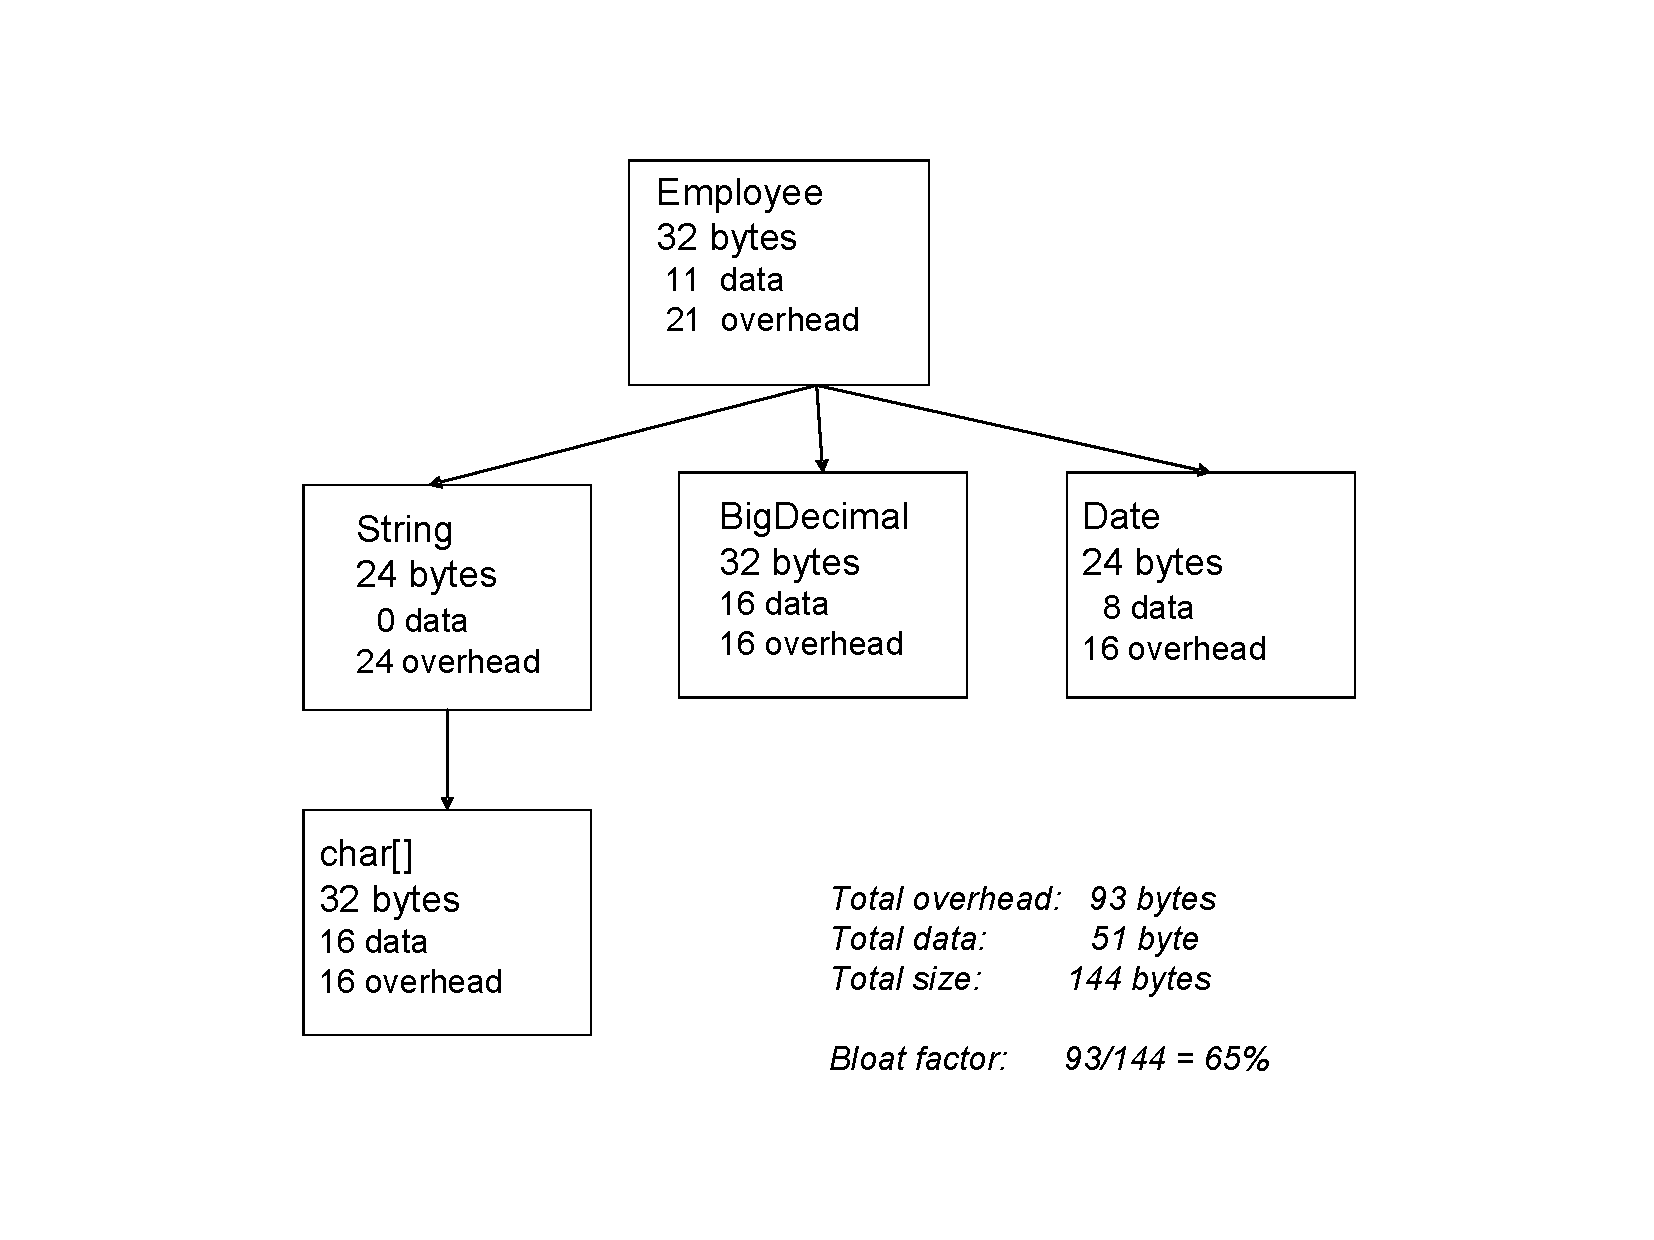
\includegraphics[width=.60\textwidth]{Figures/chapter4/employee-status.pdf}
 % 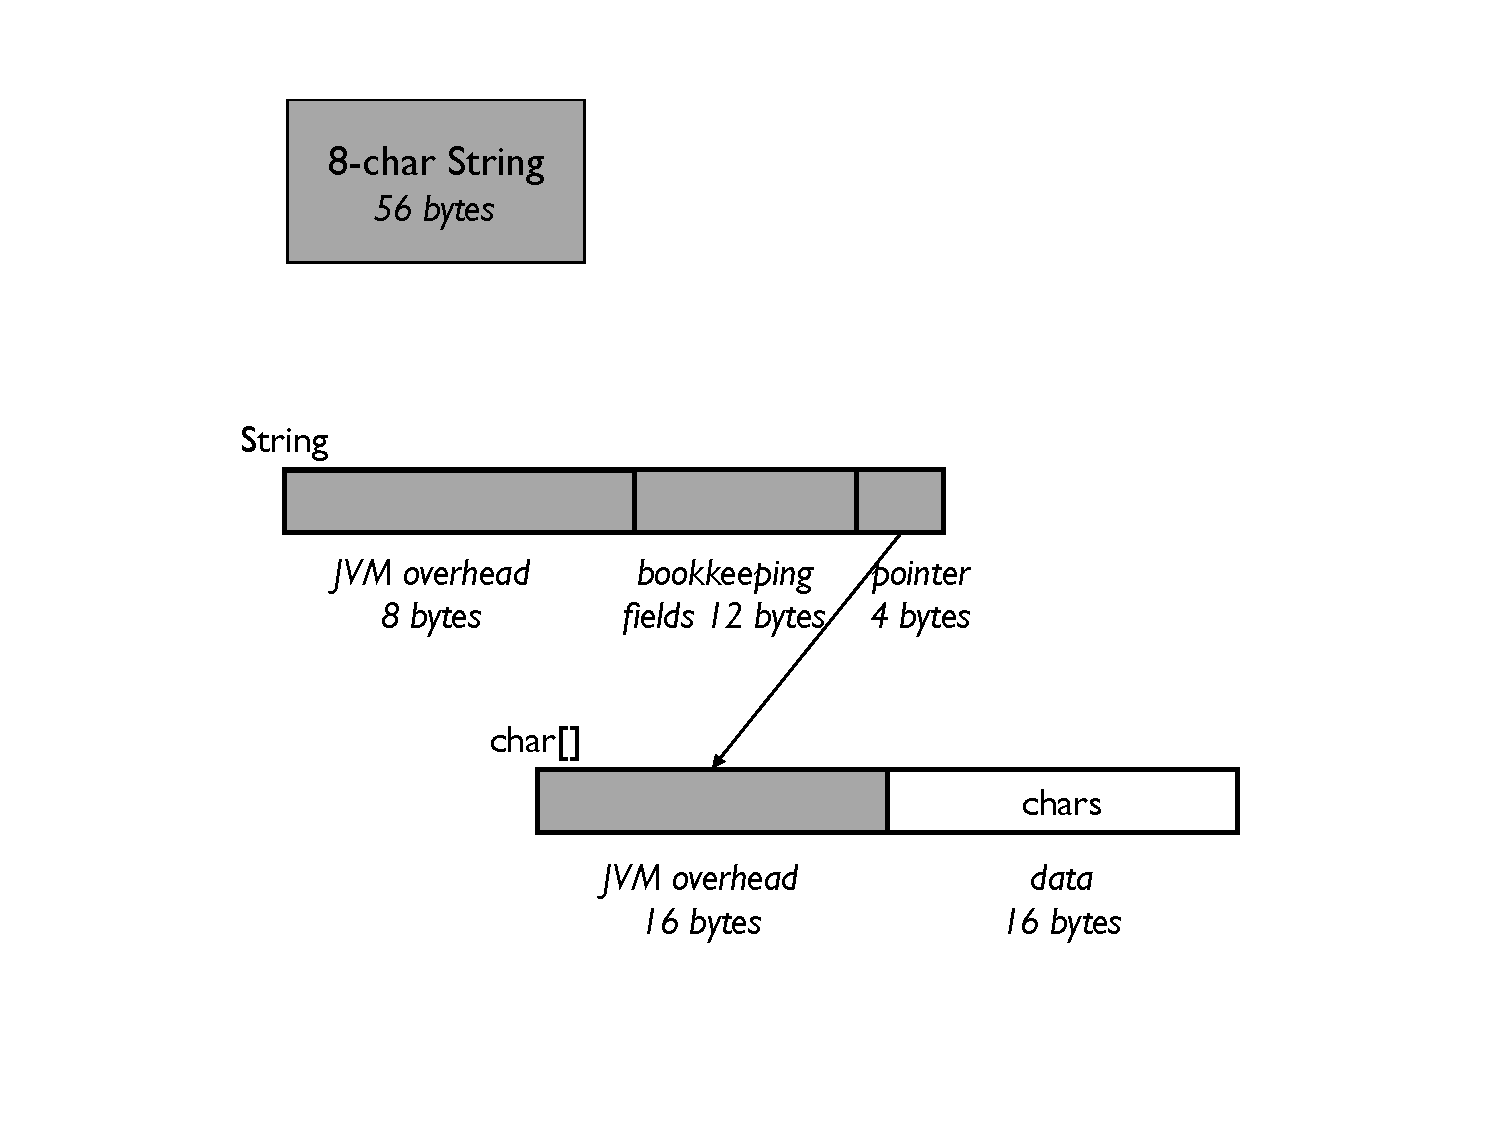
\includegraphics{eight-char-string}
  \caption{The memory layout for an employee ``John Doe"}
  \label{fig:employee-status}
\end{figure}

A comparion of this employee representation with the original \texttt{Employee} object in Section~\cite{CostOfObects} shows that the size has increased from 32 to 144 bytes, and the bloat factor, the percentage of memory overhead, has increased from 46\% to 65\%. There is more information in the new version, so it is no surprise that it is bigger. The increase in the bloat factor is more significant. Delegation increases memory bloat. Delegation introduces additional object headers, a pointer for each delegated object, and empty pointer slots for unitialized object fields. Delegation may also force additional alignment costs, since each new delegated object has to be aligned to an 8-byte boundary. 

In the spirit of keeping things simple, Java does not allow you to nest objects inside other objects, to build a single object out of other objects. You cannot nest an array inside an object, and you cannot store objects directly in an array.  You can only point to other objects. Even the basic data type \texttt{String} consists of two objects. This means that delegation is pervasive in Java programs, and it is difficult to avoid a high level of delegation overhead. Single inheritance is the only language feature that can be used instead of delegation to compose two object, but single inheritance has limited flexibility.  In contrast, C++ has many different ways to compose objects. C++ has single and multiple inheritance, union types, and variation. C++ allows you to have \texttt{struct} fields, you can put arrays inside of structs, and you can also have an array of structs.  

In Java, delegation is one of the costs you pay for object-oriented programming. This cost is often considered to be insignificant --- delegating to another object is just a single level of indirection. But the costs of the pointers and object headers needed to implement this add up quickly, and contribute significantly to large bloat factors in real applications.

\section{Fine-Grained Data Models}
\label{fine-grained-data-models}

The Java language makes it hard to avoid delegation. Programmer choices also impact delegation costs.  The current software engineering culture tends to promote delegation, and for good reasons. Delegation provides a loose coupling of objects, making refactoring and reuse easier. Replacing inheritance by delegation is often recommended, especially if the base class has a lot of extra baggage that the subclass does not need. In languages with single inheritance, once you have used up your inheritance in your single inheritance hierarchy, it becomes hard to refactor your code. In this case, delegation is more flexible than inheritance for specializing types. However, it is possible to overuse delegation, resulting in an overly fine-grained data model with many small objects. Fine-grained data models can be expensive both in execution time and memory space. 

There is no simple rule that can always be applied. Each situation has to be evaluated in context, and there may be tradeoffs among different goals. To make an informed decision, you need to understand the impact of delegation on memory requirements, by measuring the object sizes and overhead.  

 
\begin{example}[Employee emergency contact] 
An emergency contact is needed for each employee. An emergency contact is a person and a preferred method to reach her.  The preferred method can be email, cell phone, work phone, or home phone. All contact information for the contact person must be stored, just in case the preferred way does not work in an actual emergency. 
\end{example}
Here are class definitions for an emergency contact. Delegation is used heavily. This programming style is common in real applications. Often programmers are not aware of the overhead that delegation introduces. 

\ttfamily
\begin{verbatim} 
			class Employee {
        ...
        EmergencyContact contact;
			}
			
			class EmergencyContact {
        ContactPerson contact;
        Contact preferredContact;
			}
			
			class ContactPerson {
        String name;
        String relation;
        EmailAddress email;
        PhoneNumber phone;
        PhoneNumber cell;
        PhoneNumber work;
			}
			
			class Contact {
        ContactPerson owner;
			}
			
			class PhoneNumber extends Contact {
			  char[] phone = new char[10];
			}
			
			class EmailAddress extends Contact {
        String address;
			}
			
			
\end{verbatim}
\normalfont
 \begin{figure}
  \centering
 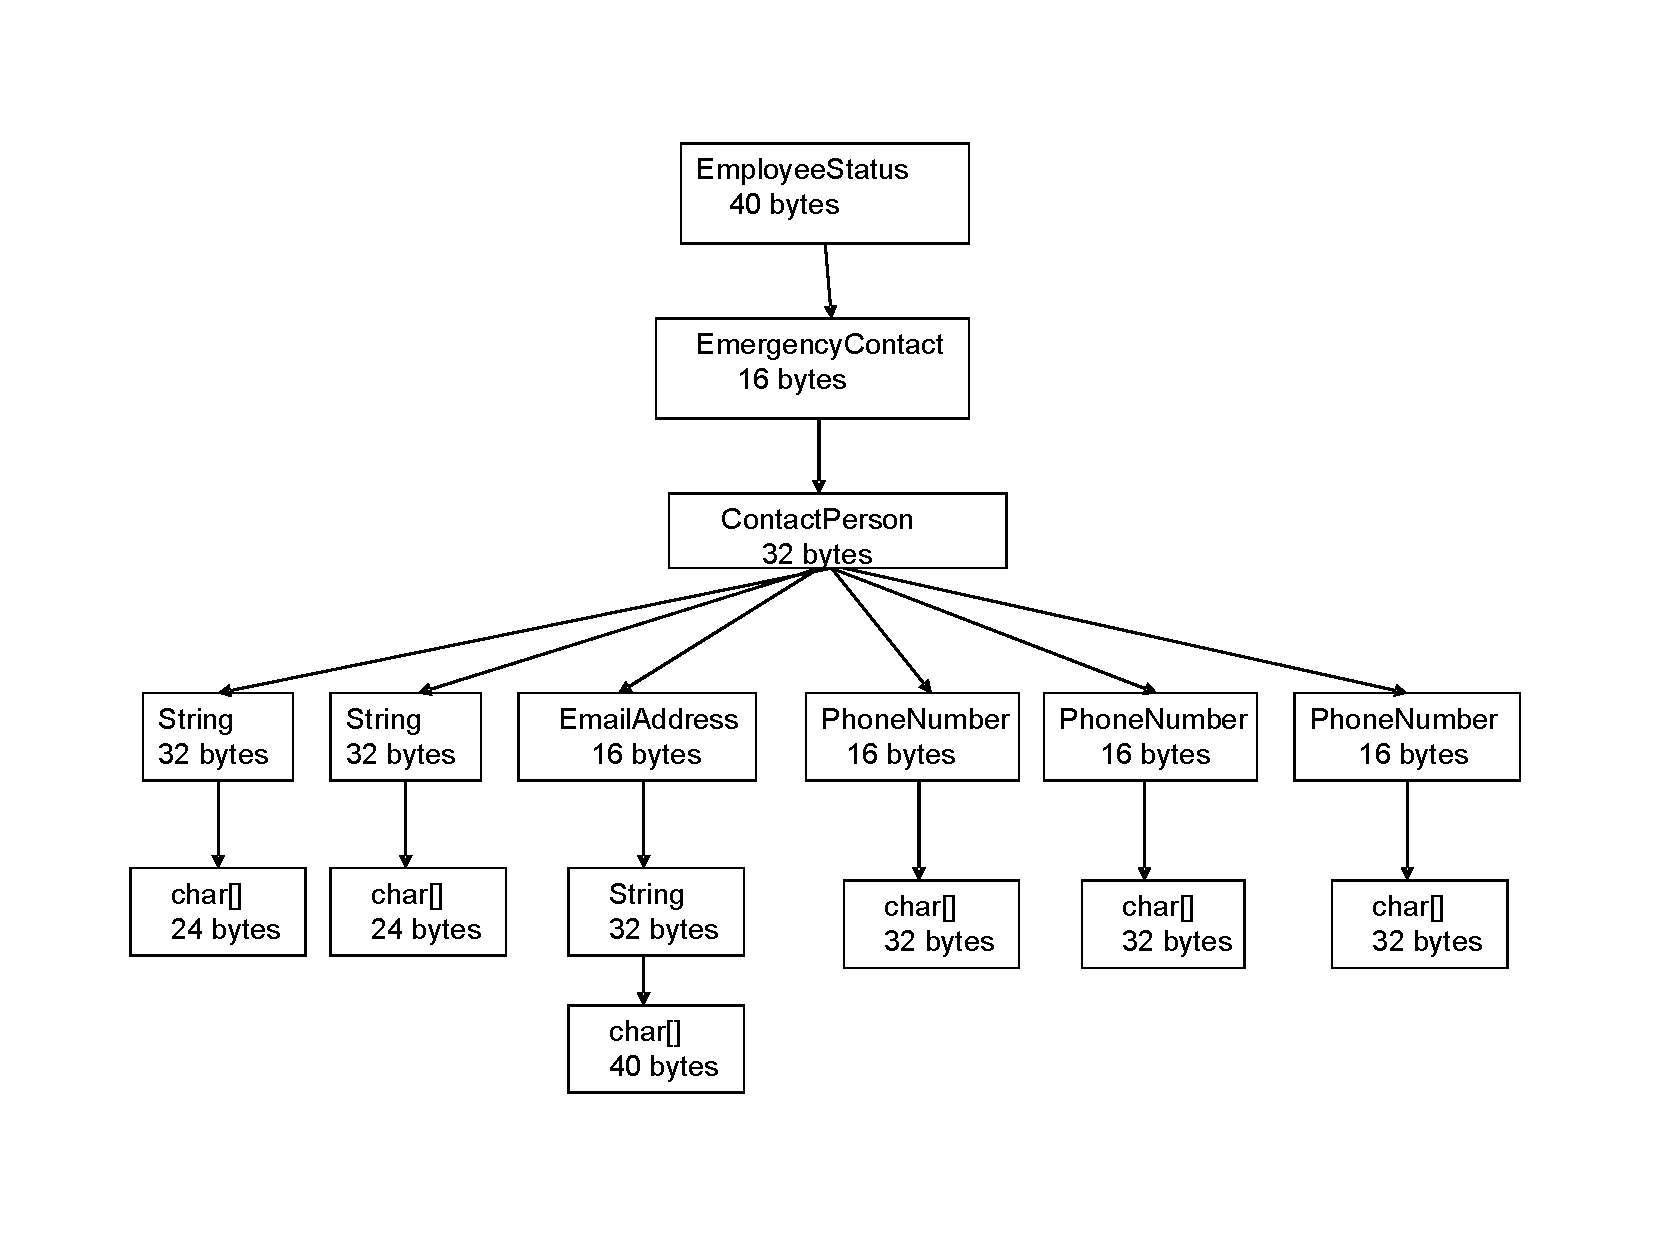
\includegraphics[width=.70\textwidth]{Figures/chapter4/employee-status-fine-grained.pdf}
 % 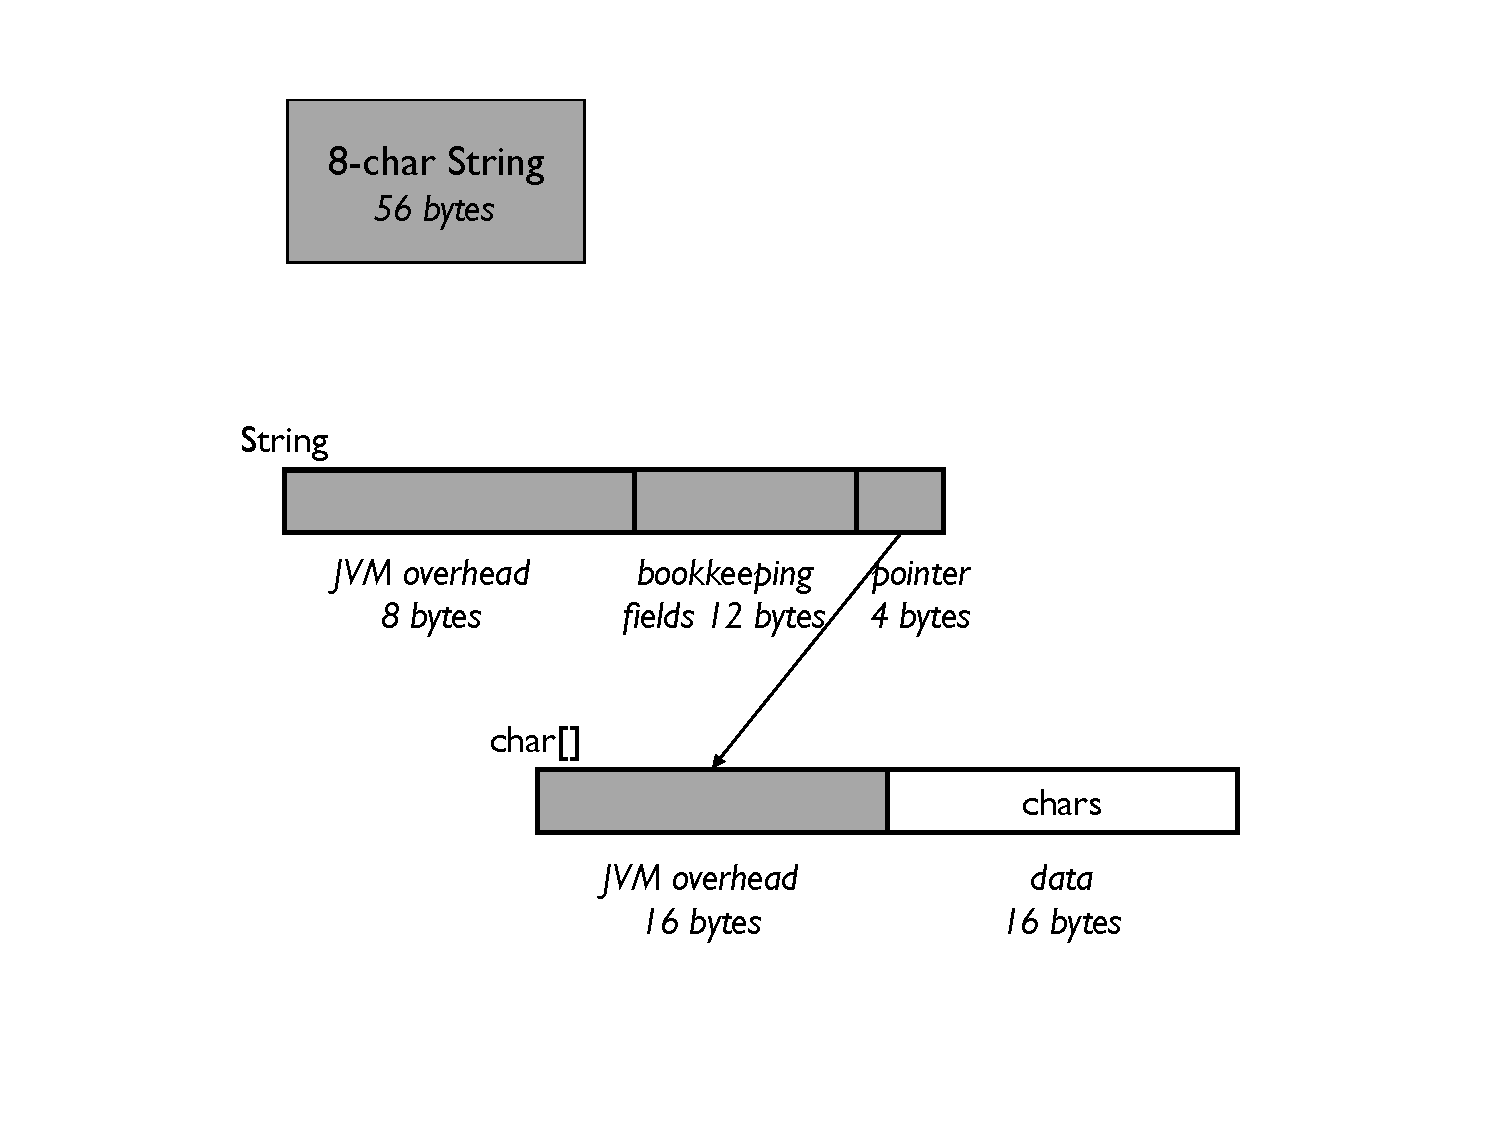
\includegraphics{eight-char-string}
  \caption{The memory layout for an employee with an emergency contact.}
  \label{fig:employee-status-fine-grained}
\end{figure}

The memory layout for a sample employee is shown in Figure~\ref{fig:employee-status-fine-grained}. There are 15 objects used to store emergency contact information. This seems excessive. The objects are all small, containing one or two meaningful fields, which is another sign of an overly fine grained data model. One object that looks superfluous is \texttt{EmergencyContact}, which encapsulates the contact person and the preferred contact method.  
Reversing this delegation involves simply inlining the two \texttt{EmergencyContact} fields into the parent \texttt{Employee} object, and then removing the \texttt{EmergencyContact} object altogether. Alternatively, it makes more sense to move the \textbf{ContactPerson} field to the Employee object, and the \texttt{preferredContact} field to the \texttt{ContactPerson}, since the preferred contact method is really an attribute of the contact person. Here is the modified code:
\ttfamily
\begin{verbatim}
	class Employee {
        ...
        ContactPerson contact;
			}
			
			class ContactPerson {
        String name;
        String relation;
        EmailAddress email;
        PhoneNumber phone;
        PhoneNumber cell;
        PhoneNumber work;
        Contact preferredContact;
			}
\end{verbatim}
\normalfont
This change eliminates an object, but not much space. You can save considerably more space by inlining the four \texttt{Contact} objects into the \texttt{ContactPerson} object, which results in a 15\%  space reduction. In a system with many in-memory \texttt{Employee}s, this reduction is significant. In order to make this change, the preferred contact method must be encoded somehow in \texttt{ContactPerson}.  A simple way to do this is to use an enumeration type field to discriminate among the different contact methods:
\ttfamily
\begin{verbatim} 
      enum PreferredContactMethod {
         EMAIL, HOME_PHONE, CELL_PHONE, WORK_PHONE;
      }
      
       class ContactPerson {
        PreferredContactMethod preferred;
        String name;
        String relation;
        String email;
        char[] cellPhone;
        char[] homePhone;
        char[] workPhone;
      }		
\end{verbatim}
\normalfont
Figure ?? shows the memory layout after these changes.

When many objects are used to represent a single entity, this is an indication that the data model may be using too much delegation. Delegation is good, but it is possible to overuse a good thing. A design with fewer, bigger objects has less overhead and is more scalable. 

\section{Large Base Classes}

For cross-cutting features that are common to many objects, inheritance is an obvious implementation choice. A base class implements a feature, and all objects that require the feature are instances of subclasses of this base class. 

\begin{example}[Keeping track of updates] 

A frequent data management requirement is to track creation and update information, that is, when data is created or updated and by whom.  Here is a base class that stores create and update information, taken from a real application.  
\ttfamily
\begin{verbatim}
      class ModifyInfo {
         Date createDate;
         Party enteredBy;
         Date updateDate;
         Party updateBy;
      }
\end{verbatim}
\normalfont
It is now possible to track changes to any object by subclassing from \texttt{ModifyInfo}. 
\end{example}
Returning to Example 3 in Section~\ref{fine-grained-data-models}, suppose that updates to employees' emergency contacts need to be tracked. You have to be a bit careful here. If you decide to use the fine-grained data model, and decide to track changes to every contact phone number or email address, you may run out of memory. As shown in Figure~\ref{}, this adds an extra 16 bytes to each \texttt{Contact} object, and up to four additional \texttt{Date} and \texttt{Party} objects for each of the four \texttt{Contact} object. A far more scalable solution is to track changes to each \texttt{ContactPerson}, whether or not you stay with the fine-grained data model. 

When highly-delegated objects are combined with large base classes, memory costs multiply quickly. 
you may end up with many big objects


The moral of this example is that if you have both a fine-grained design and large base classes, memory costs can multiply quickly. The resulting of fine-grained functionality may not be necessary, or even intended. For example, it is overkill to attach update information to every contact point for every emergency contact for every employee. It is probably sufficient to keep update information only for the \texttt{ContactPerson}. 

It is very easy for a programmer to subclass without looking closely at the memory size of a superclass, especially if the inheritance chain is long. Also, programmers may not think about how many instances of an entity will be created at runtime. The only thing worse than too many small objects is too many big objects. 

\section{64-bit Architectures}

n th 64-bit world, that string is now 96 bytes, and the reason is 50\% larger than it was in 32-bit JVM. The reason is first of all So in this case, just the delegation costs is now 32 bytes, which is basically 1/3 of the cost, and the total cost of the string is up by 50\%.  In general, this is a real problem for fine-grained designs. Unfortunately, a lot of designs out there are fine0grained, and we'll see the reasons for that. 


So just lets talk a little about what this means for 64-bit JVMs. People are busting out of this 32-bit address space now, and they are saying let's go to 64-bit, and that will solve everything. Unfortunately, when you go to 64-bit, things blow up pretty quickly. , the object headers are double, pretty sure that's the same thing in sun. arrays are not quite double. 24 bytes. The other thing is that all the pointers instead of being 4 bytes, are now 8 bytes; and finally, there's still that same alignment cost in J9. In SUN you will have a higher alignment cost, since in SUN now it's aligned to 8-byte boundary, where it was aligned to 4-byte boundary before.  The studies I've read, both outside and inside IBM, are showing that going to a 64-bit JVM will increase your memory usage by 40-50\%, and I've heard arguments that say that yur application will run faster, because of the native architecture and all that,  but in some cases there is evidence that it may run slower, because of the worse cache locality. It's another example where it's super important to measure, and not make assumptions that this will fix my speed problem, or it will fix my memory problem. There are a lot of surprises in this area. So J9, and some of the other JVMs, I don't think SUN has this yet, I coud be wrong, I know JRocket has it , they have a mode have called compress addressing, where they can squeeze a few extra bits out of the 32-bit addresses, and in J9 6SR2 is going to allow addressing of up to 28 gig with a 32 bit address still, so without all of these additional footprint problems, if you use this compressing flag. From what I've read, it's only a few percentage degradation in performance, it's pretty minor, so it can certainly help people in this transition area.




\section{Summary}
